\documentclass[runningheads,a4paper]{llncs}
\usepackage{amssymb}
\setcounter{tocdepth}{3}
\usepackage{listings}
\usepackage{booktabs}
\usepackage{mathtools}
\usepackage{tabularx}
\usepackage{fixltx2e}
\PassOptionsToPackage{hyphens}{url}\usepackage{hyperref}
\usepackage[hyphens]{url}
\usepackage{upquote,textcomp}
\lstset{breaklines=true, basicstyle=\scriptsize\ttfamily, upquote=true}

\usepackage{fancyvrb}
\VerbatimFootnotes
\usepackage{cprotect}

\usepackage{graphicx}
\makeatletter
\def\maxwidth#1{\ifdim\Gin@nat@width>#1 #1\else\Gin@nat@width\fi}
\makeatother

\usepackage{amsmath}
\usepackage{pmml-new}

\usepackage{color,graphics,array,csscolor}

\usepackage{fontspec,unicode-math}
\usepackage[Latin,Greek]{ucharclasses}
\setTransitionsForGreek{\fontspec{Times New Roman}}{}

\usepackage{subscript}
\lstset{breaklines=true, basicstyle=\scriptsize\ttfamily}

\begin{document}
\mainmatter

\title{Methinks: Enabling Sophisticated Comment Management in the Social Web}
\titlerunning{Methinks}
\author{Giorgos Flouris\inst{1} \and
Theodore Patkos\inst{1} \and
Ilia Adami\inst{1} \and
Antonis Bikakis\inst{2} \and
Manos Dimitrakis\inst{1} \and
George Mathioudakis\inst{1} \and
Giannis Roussakis\inst{1} \and
Dimitris Plexousakis\inst{1}}
\authorrunning{Giorgos Flouris et al.}
\institute{FORTH, Greece\and
UCL, UK\\
\email{fgeo@ics.forth.gr, 
patkos@ics.forth.gr, 
iadami@ics.forth.gr, 
a.bikakis@ucl.ac.uk, 
mdimitrak@ics.forth.gr, 
gmathiou@ics.forth.gr, 
rousakis@ics.forth.gr, 
dp@ics.forth.gr}}
\maketitle

\begin{abstract}
User reviews, comments and votes on the Social Web form the modern version of word-of-mouth communication, which has a huge impact on people's shopping habits, businesses and the overall market. Despite that, systems have so far limited practical success in helping consumers and businesses analysing, managing and understanding Social Web content. In this paper, we present a new tool that leverages a combination of techniques from Semantic Web, Computational Argumentation and Crowdsourcing to support this activity, through an intuitive and functional user interface.

\keywords{Comments, Computational Argumentation, Crowdsourcing, Reviews, Semantic Web, Social Web}
\end{abstract}


\section{Introduction}

The Social Web is populated with arguments, which usually have the form of comments, opinions or reviews, and are the main ingredients of online discussion forums, social networks, online rating and review sites, debate portals and other online communities - the electronic version of word-of-mouth communication. Since the emergence of the Social Web, its impact has been paramount to several aspects of human behaviour, ranging from health-related  \cite{_Ref490737972}, to buying  \cite{_Ref490738051}, travelling  \cite{_Ref490738065} or voting habits  \cite{_Ref490738076}. Also, opinions in the Social Web significantly impact businesses and the overall market; a study on the impact of online reviews on the restaurant industry found that a one-star increase in Yelp.com rating led to a 5-9\% increase in the revenue of the rated restaurants  \cite{_Ref490738087}.

It is thus clear that understanding, analysing and managing such comments is of paramount importance in various industrial sectors. Towards this end, two main approaches exist. On the one end, Computational Argumentation  \cite{_Ref490738126} has provided mature results in understanding and formalizing the interplay of arguments in structured debates. This work has yet limited applicability on the Social Web, due to the highly unstructured nature of the latter, despite some recent efforts to bridge the differences  \cite{_Ref490738134},  \cite{_Ref490738141}. On the other end, opinion analysis methods attempt to make sense out of online discussions, relying heavily on Natural Language Processing (NLP) techniques. Their performance in understanding the basic trends and sentiments of online dialogues has improved remarkably over the last years, yet their accuracy is still very low when it comes to identifying the arguments in opinions, understanding their relations (attack/support), or extracting the most acceptable arguments in a dialogue  \cite{_Ref490738149}.

The Methinks system aims to bring these two approaches closer, by harnessing crowdsourcing techniques instead of NLP for obtaining meta-information about an opinion and by relying on Semantic Web and Computational Argumentation methods to automate opinion processing. The novelties reside both at the frontend, where a number of features have been developed to facilitate the task of comment annotation for the {\em consumer} (typically a potential customer searching for a product or service, having the role of comment reader or writer), and at the backend where novel, powerful and semantically-enriched analytical tools have been developed to assist the {\em analyst} (typically an employee of the product or service provider, a system administrator, or a market analyst) in the task of spotting valuable comments and ironing out irrelevant or unhelpful ones. Eventually, the experience of all beneficiaries is improved by a more elaborate characterization of comments in terms of acceptance of the opinions they express by the participants of a given dialogue, and quality of their content.

\section{Features of Methinks}

\subsection{General Properties}

Methinks is an online service developed using modern web technologies, intended to be licensed and delivered as Software as a Service (SaaS). The target market of Methinks includes, among others, hotels, online booksellers, listings directories (e.g., booking.com, ebay, etc.) and content aggregators.

Unlike generic commenting and debating tools such as Disqus\footnote{ https://disqus.com/}, the objectives of Methinks are very much market-related, namely to (a) assist the consumer towards {\em more informed shopping decisions}, and (b) help the analyst identify {\em trends}, as well as {\em problematic or attractive characteristics} of the offered products or services to improve their business. Each objective is achieved through a different frontend operating on the same backend\footnote{ Consumer interface: http://139.91.183.40:8080/methinks-dev/demo/ (some features require login; you may create your own account, or use the name: demo\_user@demo.com with password: demo\_user).

Analyst interface: http://139.91.183.40:8080/methinks-dev/admin/\#!/login (username: admin@admin.com, password: admin1234).}.

For the User Interface design of the final prototype, the user-centred design (UCD) process  \cite{_Ref490738642} was followed to ensure optimal usability of the end product. The process included the following phases: user requirement collection and analysis, creation of high-fidelity interface mock-up designs, expert walkthrough evaluation of the prototypes, adjustments based on expert evaluation results, user-based evaluation in a laboratory environment, and further adjustments of the prototype based on the results from the evaluation.

\subsection{Features for the Consumer}

\subsubsection{Comments as first-class citizens}

In Methinks, comments are organised in user-generated {\em topics}. For example, in the provided demo (referring to the hotel domain), different topics may include ``restaurant'' and ``room''; however, the list of topics is open, to allow the comment writers to give emphasis on any aspect that they consider important (e.g., ``mosquitos'' or ``nightlife'').

One of the main ideas behind Methinks is that comments are treated as {\em first-class citizens}, carrying as much information as the actual description of a product or service. A button brings about a drawer showing the provided comments, with various options for searching, filtering, organising or viewing them (see Fig.~\ref{_Ref490739495}). The related retrieval functionalities are implemented using SPARQL queries posed against an RDF backend following an appropriate ontological schema.
\begin{figure}[h!]
\centering
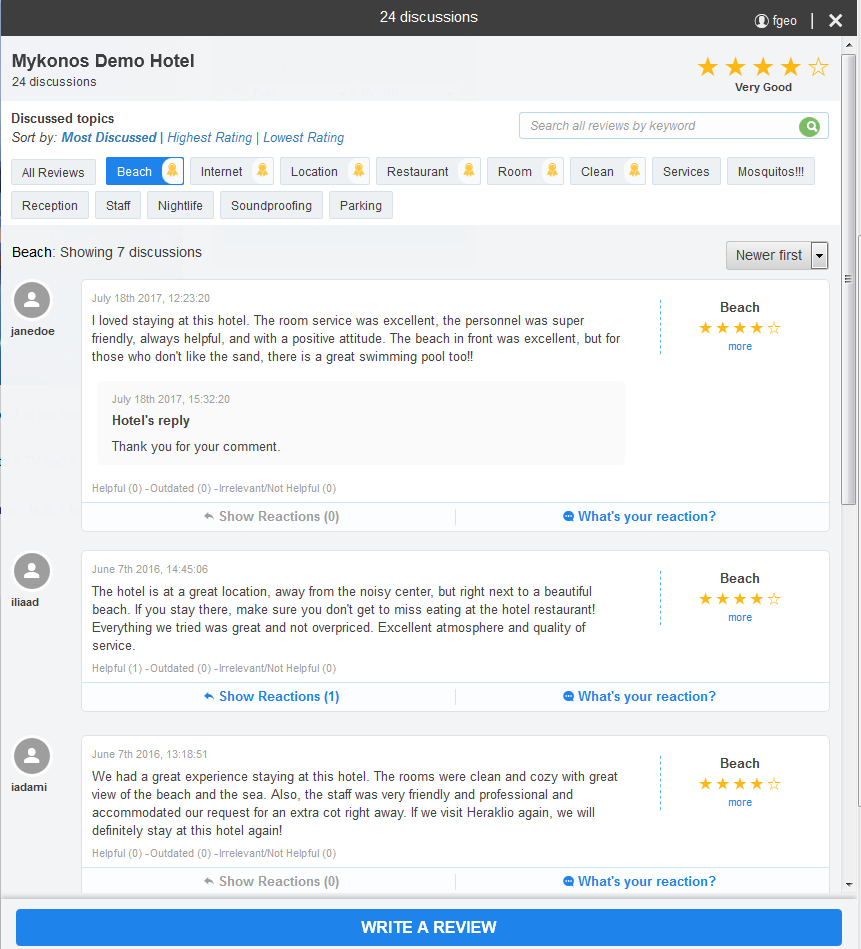
\includegraphics[width=\maxwidth{\textwidth}]{./img/image1.png}
\cprotect\caption{  The  Drawer (Main Methinks Window)}
\label{_Ref490739495}
\end{figure}


More importantly, comments are {\em integrated} with the actual page content. Any textual content in the description of the product/service that corresponds to an existing topic of discussion appears underlined in an indication that there is further information linked to it. On mouse-over, a box appears above the underlined text showing the number of discussions that have been created on this particular topic (see Fig.~\ref{_Ref490743450}). Upon clicking inside the box, the main Methinks plug-in window (Fig.~\ref{_Ref490739495}) expands and shows the discussions that are associated with the selected topic. Similarly, selecting some text in the description, allows one to search in the comments for this text, or create a new topic for this text.
\begin{figure}[h!]
\centering

\includegraphics[width=\maxwidth{\textwidth}]{./img/image2.png}
\cprotect\caption{ Integration  of Comments in Web Page Content}
\label{_Ref490743450}
\end{figure}


\subsubsection{Leveraging crowdsourcing and argumentation to understand comments}

Whenever a consumer wants to add a comment to the system, this can appear as a new comment, or as a {\em reaction} to an existing one. In both cases, the comment writer needs to provide topics (existing or new ones), and may additionally provide various types of textual and/or structured feedback. The system provides help in selecting topics, by proposing existing topics that match what the user is writing.

Textual feedback is addressed to humans, whereas structured feedback (like votes, star ratings and characterizations of aspects as outdated or helpful) helps evaluating the comments and the product/service. In fact, users have various ways to criticise (or praise) various aspects of previously submitted comments or of the product/service under discussion, and this rich feedback is leveraged by complex argumentation-inspired algorithms, whose details can be found at  \cite{_Ref490741703}. These algorithms allow a fine-grained analysis of how positively or negatively the crowd views certain aspects associated with the product/service at hand, or the comment itself, by leveraging (among other things) the two types of relations among comments (attack/support) using methods from quantitative argumentation frameworks  \cite{_Ref490738141}, as well as by employing the categorization of feedback in different aspects and/or topics.

Comments are evaluated by assessing their {\em quality} and {\em acceptance}. The quality rating of a comment determines its reliability and usefulness for other consumers and helps in ranking the comments. The acceptance rating is used to determine whether other consumers agree with the comment's assessment on the topic (positive or negative); this in turn determines the contribution of the comment in formulating the final score assigned to the topic. NLP technologies may help improve these algorithms in the future; yet, our goal on involving users in the loop aims at keeping them engaged in the reviewing process.

\subsection{Features for the Analyst}

With regards to the analyst, we have developed a rich graphical user interface (GUI) allowing monitoring trends and understanding the social feeling associated with products (see Fig.~\ref{_Ref490743665}). The analyst interface allows {\em moderating} (accepting/rejecting) comments, thereby allowing the analyst to block comments with offensive or profane language, and control what comments are published to the webpage. It also allows {\em responding} to comments, a feature that gains popularity in most review sites. More importantly, it provides various {\em visualizations} of the comments'/topics' quantity and scores. All visualizations allow various types of organisation and filtering along various dimensions (temporal, topical, status etc), leveraging the flexibility of our semantic representation and facilitated by SPARQL expressiveness.
\begin{figure}[h!]
\centering
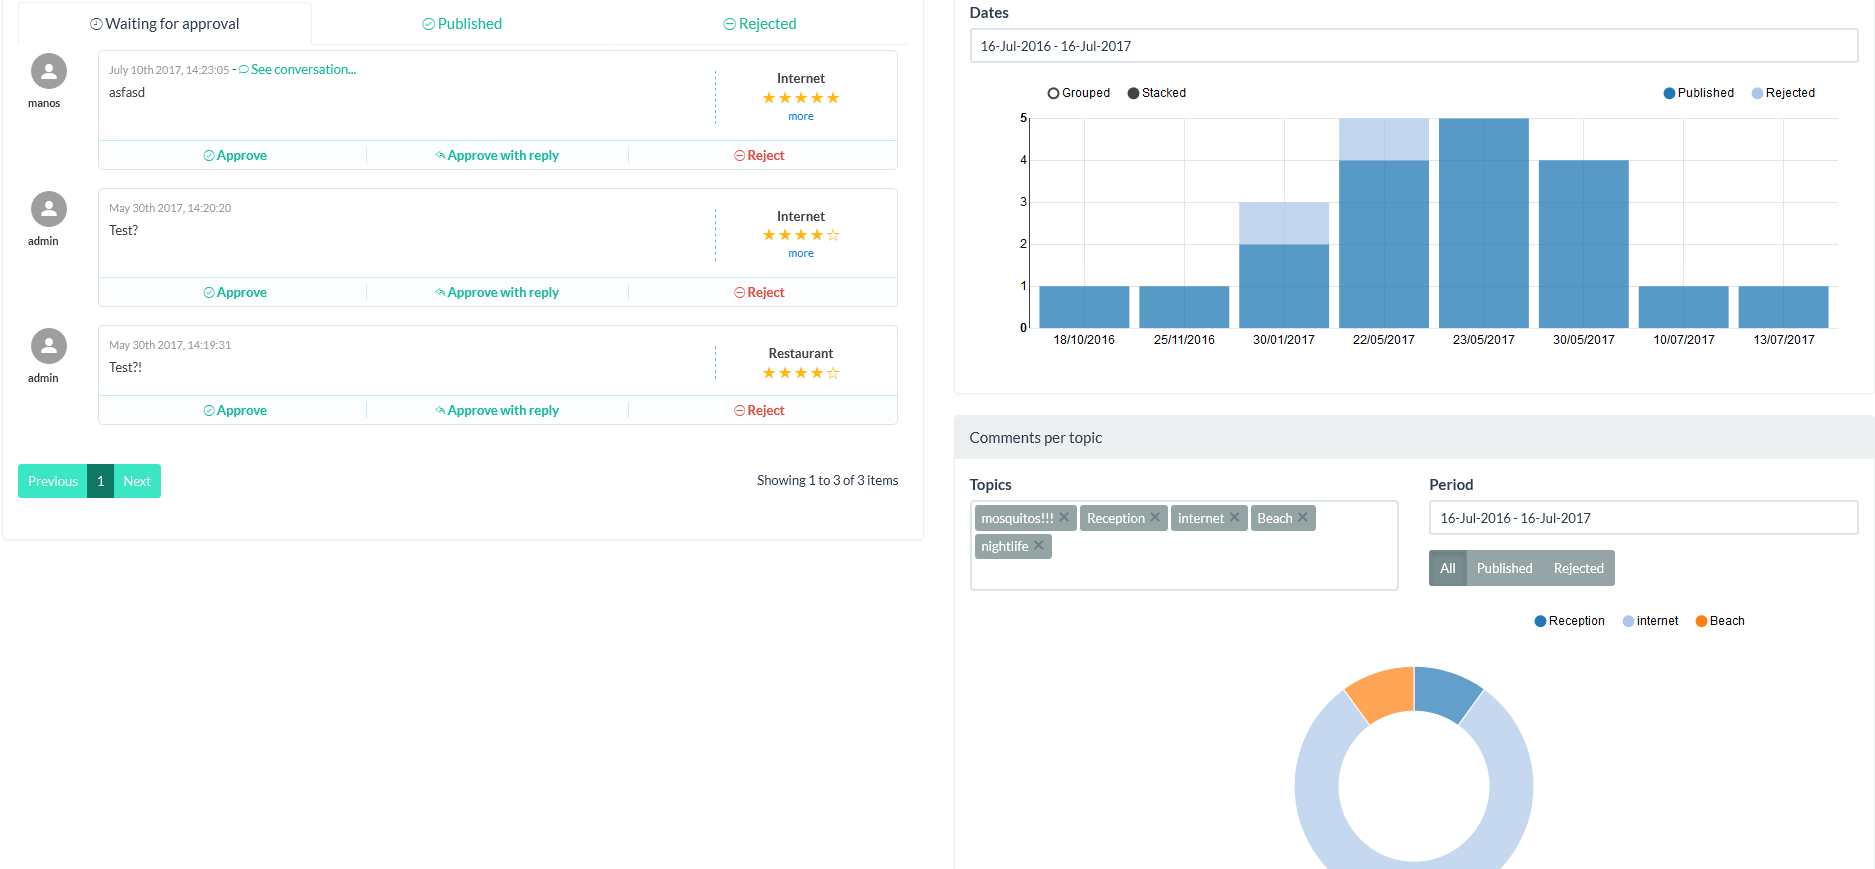
\includegraphics[width=\maxwidth{\textwidth}]{./img/image3.png}
\cprotect\caption{ The User Interface for the Analyst}
\label{_Ref490743665}
\end{figure}


\subsection{Used Technologies}

The frontend was implemented as a web-page plugin using the AngularJS\footnote{ https://angularjs.org} framework. It was designed and developed with the following two principles in mind: easy web-page integration and minimum possible dependencies on external javascript and styling libraries.

The analyst interface was implemented as a single-page application in order to provide a user experience similar to that of a desktop application. It was developed on top of AngularJS framework, using Twitter Bootstrap\footnote{ http://getbootstrap.com} for the styling and positioning of the UI  components. The various analytics graphs are created dynamically as SVG images with the help of the nvd3\footnote{ http://nvd3.org} and D3.js\footnote{ https://d3js.irg} libraries.

The backend uses Virtuoso Triplestore\footnote{ https://virtuoso.openlinksw.com} version 7.2 to store all the created comments along with all the metadata (e.g., creation date, authors, comment relations etc.) that are necessary for supporting Methinks' functionalities. The storage and data access layers are implemented using RDF and SPARQL, respectively.

Even though Methinks' data could conceivably be stored also using relational technologies, the use of semantics allows future interoperability among different deployments of the Methinks platform and datasets from the Data Web, therefore allowing better integration and paving the road for future developments that could lead to a global repository of annotation-rich comments, where comments from different web sites and products/services could be combined with online data to provide a more complete user experience.

The ontology used for the representation of the comments transfers part of the business logic to the representation layer, for easier maintenance, and is shown in Fig.~\ref{_Ref490744387}. The ontology design employed a functionality-oriented approach. In particular, the top-level concepts (O1\_Creation\_Data, O2\_Strength, O3\_Concept) were created with regards to the types of properties that different lower-level concepts should support. For example, the class O1\_Strength is the domain of all properties associated with the notion of strength (acceptability, quality, etc.) and subsumes all concepts whose value (strength) is evaluated in the system (namely, topics and various types of arguments). The same idea is used for the other concepts. More details are omitted due to lack of space.
\begin{figure}[h!]
\centering
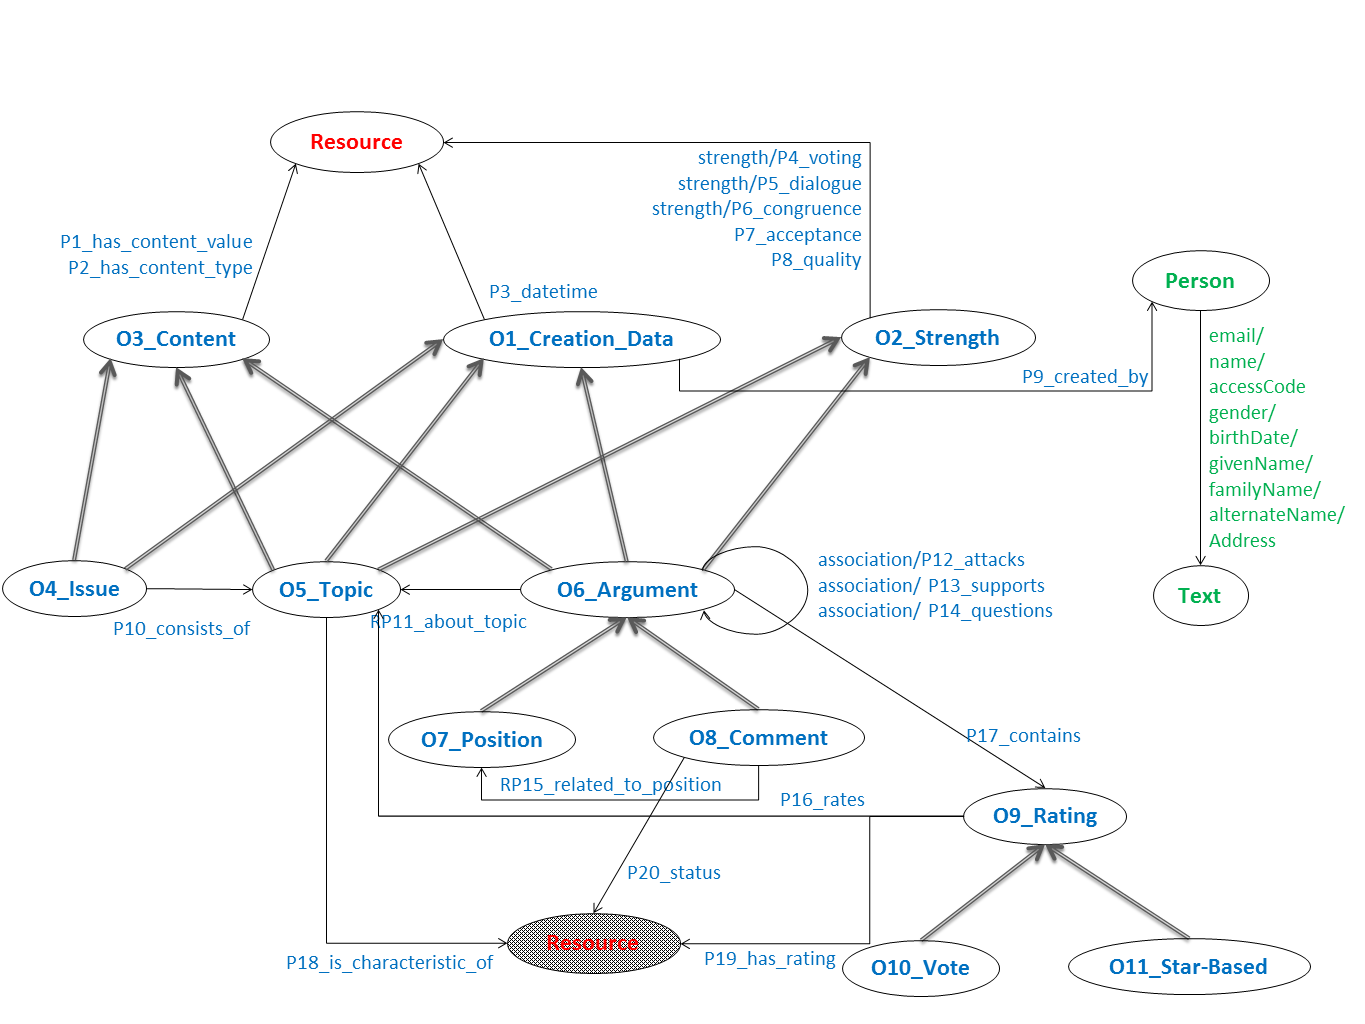
\includegraphics[width=\maxwidth{\textwidth}]{./img/image4.png}
\cprotect\caption{ The Methinks Ontology}
\label{_Ref490744387}
\end{figure}


\section{Conclusion}

In this paper, we presented {\em Methinks}, a tool for enhanced review sites that allows easier management and analysis of user comments in a Social Web context. Emphasis is given to market-related web sites, providing features that create benefit for both the consumer and the product/service provider. The tool is still under development, and various new features are considered, such as the introduction of multimedia comments, cross-website and/or cross-product comparison using comment scores and others.

\begin{thebibliography}{4}

\bibitem{_Ref490738051} C.M. Cheung, D.R. Thadani. The impact of electronic word-of-mouth communication: A literature analysis and integrative model. Decision Support Systems 54(1):461--470. 2012.
\bibitem{_Ref490738642} D.A. Norman, S.W. Draper. User-centred System Design: New Perspectives on Human-Computer Interaction. L. Erlbaum Associates Inc., 1986.
\bibitem{_Ref490738149} M. Lippi, P. Torroni. Argumentation Mining: State of the Art and Emerging Trends. ACM Transactions on Internet Technology 16(2)10, March 2016. 
\bibitem{_Ref490738087} M. Luca. Reviews, reputation, and revenue: The case of yelp.com. Technical Report 12-016, Harvard Business School. 2011.
\bibitem{_Ref490738141} P. Baroni,  M. Romano,  F.  Toni,  M.  Aurisicchio,  G. Bertanza. Automatic evaluation of design alternatives with quantitative argumentation. Argument \& Computation 6(1):24--49, 2015.
\bibitem{_Ref490738126} P. Besnard, A. Hunter. Elements of Argumentation. The MIT Press. 2008.
\bibitem{_Ref490738065} Q. Ye, R. Law, B. Gu, W. Chen. The influence of user-generated content on traveller behaviour: An empirical investigation on the effects of e-word-of-mouth to hotel online bookings. Computers in Human Behaviour 27(2):634--639. 2011.
\bibitem{_Ref490738076} R.M. Bond, C.J. Fariss, J.J. Jones, A.D.I. Kramer, C. Marlow, J.E. Settle, J.H. Fowler. A 61-million-person experiment in social influence and political mobilization. Nature 489(7415):295--298, 2012.
\bibitem{_Ref490738134} S. Eilmez, J. Martins, J. Leite. Extending social abstract argumentation with votes on attacks. In Theory and Applications of Formal Argumentation, pages 16--31, 2014.
\bibitem{_Ref490741703} T. Patkos, G. Flouris, A. Bikakis. Symmetric Multi-Aspect Evaluation of Comments (Extended Abstract). ECAI-16, 2016.
\bibitem{_Ref490737972} W.-y.S. Chou, A. Prestin, C. Lyons, K.y. Wen. Web 2.0 for health promotion: Reviewing the current evidence. American Journal of Public Health 103(1):e9--e18, 2012. 

\end{thebibliography}

\end{document}